\newpage\section{Introduction}

The role of information systems in modern business solutions is indisputable, [...] Developing such a solution is the goal of this work \parencite{venkatesh_usability_2014}. 

\newpage\section{Foundations}

Process mining needs to access [...] and used by many large-scale companies \parencite{hoehle_espoused_2015} across the world.


\subsection{A sub-section}
\begin{figure}[h]
    \centering
    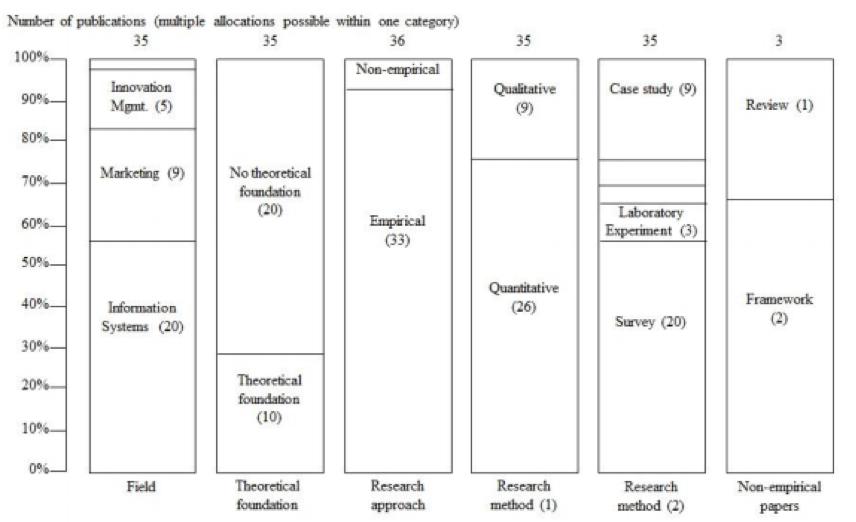
\includegraphics[width=0.8\textwidth]{content/00_template/images/Picture1.png}
    \caption{Analysis of identified Papers}
    \label{fig:mesh1}
\end{figure}

The work of \textcite{hoehle_espoused_2015} provides a solution for this problem in terms of [..].

\subsection{Yet another sub-section}

As you can see in the figure \ref{fig:mesh1}, everything looks better in a diagram. Also, in the page \pageref{fig:mesh1} 
is the same example.

\newpage\section{Methodology}

A solution for the aforementioned problem can be achieved by developing a software  [...] would be able to start process mining tasks using this event log \parencite{hoehle_espoused_2015, venkatesh_usability_2014}.

\newpage\section{Results}

Currently only few tools are focusing [...]  The findings in this area will be covered and be used to draw the essential requirements of the final solution. 

\subsection{Citation examples}

And here we demonstrate like \parencite{hoehle_espoused_2015} how citations look alike in this \LaTeX file. You can also list all authors \parencite{venkatesh_usability_2014}. And click any of the references and see what happens in your PDF reader, like here: \textcite{university_of_arkansas_mobile_2015}.

\newpage
\section{Conclusion}

Giving the conclusion here.

 \subsection{Summary of findings}

Here is a sample table. 

\begin{table}[h!]
\centering
\begin{tabular}{|p{2cm}|p{2cm}|p{4.5cm}|p{2cm}|}
\hline
\multicolumn{1}{|c|}{\textbf{Survey}} &
  \multicolumn{1}{c|}{\textbf{Construct}} &
  \multicolumn{1}{c|}{\textbf{Item Used}} &
  \multicolumn{1}{c|}{\textbf{Source}} \\ \hline
\multirow{6}{*}{\textbf{\begin{tabular}[c]{@{}l@{}}Job \\ (Survey 1)\end{tabular}}} &
  \multirow{2}{*}{***} &
   &
  \multirow{2}{*}{} \\ \cline{3-3}
 &                      &  &                   \\ \cline{2-4} 
 & \multirow{4}{*}{***} &  & \multirow{4}{*}{} \\ \cline{3-3}
 &                      &  &                   \\ \cline{3-3}
 &                      &  &                   \\ \cline{3-3}
 &                      &  &                   \\ \hline
\multirow{3}{*}{\textbf{\begin{tabular}[c]{@{}l@{}}General \\ (Survey 2)\end{tabular}}} &
  \multirow{3}{*}{***} &
   &
  \multirow{3}{*}{} \\ \cline{3-3}
 &                      &  &                   \\ \cline{3-3}
 &                      &  &                   \\ \hline
\end{tabular}
\caption{Sample table}
\label{tab:sampletable}
\end{table}

\subsection{Limitations}
\subsection{Recommendations for future research}